\section{Gestión del tiempo}
\subsection{Planificación de la gestión del tiempo}
\label{plan:time}
Una vez se hayan conocido los requerimientos y se hayan realizado las
entrevistas oportunas, se procederá a definir la gestión del tiempo del
proyecto. No obstante, se evitará invertir demasiado tiempo y esfuerzo en
esta parte, debido a que al no haber realizado ningún otro proyecto similar
sobre el que basar las estimaciones, la estimación general del proyecto será
imprecisa, incorrecta y estará llena de desviaciones. En cambio, el esfuerzo
se focalizará en el apartado de seguimiento y control de esta parte.

\subsection{Definición de las actividades}
\begin{enumerate}

 \scriptsize
  \item Crear estructura del documento de \LaTeX .
  \item Planificación.

  \begin{enumerate}

    \item Alcance

    \begin{enumerate}

      \item Documentar la gestión del alcance.
      \item Documentar la gestión de los requerimientos.
      \item Documentar la gestión de la validación del alcance.
      \item Escribir un borrador con las preguntas a realizar en las
        entrevistas.
      \item Realizar entrevistas.

      \begin{enumerate}

        \item Realizar entrevista con los trabajadores de desarrollo.
        \item Realizar entrevista con los trabajadores de gestión.
        \item Realizar entrevista con los trabajadores de contabilidad.

      \end{enumerate}

      \item Procesar respuestas y elaborar los requerimientos.
      \item Generar un alcance inicial.
      \item Convocar una reunión con los interesados para validar el alcance.
      \item Corregir los requerimientos y el alcance.
      \item Documentar la gestión del seguimiento y control del alcance.
      \item Generar un \gls{edt}.

    \end{enumerate}

    \item Tiempo

    \begin{enumerate}

      \item Documentar la gestión del tiempo del proyecto.
      \item Realizar una definición de actividades.
      \item Analizar y elaborar una secuencia de actividades.
      \item Estimar la duración de las actividades.
      \item Identificar y recoger los hitos.
      \item Realizar un diagrama de Gantt.
      \item Redactar la gestión del seguimiento y control de las actividades.

    \end{enumerate}

    \item Calidad

    \begin{enumerate}

      \item Documentar la gestión de la calidad del proyecto.
      \item Especificar qué es considerada como calidad mínima y qué como
        calidad añadida.
      \item Redactar la gestión del seguimiento y control de la calidad.

    \end{enumerate}

    \item Riesgos

    \begin{enumerate}

      \item Documentar la gestión de los riesgos del \gls{pfm}.
      \item Analizar y elaborar una lista de posibles riesgos.
      \item Elaborar planes de contingencia.

    \end{enumerate}

  \end{enumerate}

  \item Gestión
  \label{item:gestion}

  \begin{enumerate}

    \item Realizar seguimiento y control del alcance.
    \item Realizar seguimiento y control del tiempo.
    \item Realizar seguimiento y control de la calidad.
    \item Realizar seguimiento y control de los riesgos.

  \end{enumerate}

  \item Diseño
  \label{item:diseno}

  \begin{enumerate}

    \item Realizar un \gls{modentrel} del dominio.
    \item Diseñar y documentar la \gls{api}. \label{item:disdocapi}

  \end{enumerate}

  \item Desarrollo

  \begin{enumerate}

    \item Formación

    \begin{enumerate}

      \item Obtener información de los aspectos básicos de las \gls{api}.
      \item Aprender los fundamentos del \gls{tdd}.
      \item Aprender a usar el \gls{webframework} \textit{Symfony}
        \footnote{\url{https://symfony.com/}} con \gls{api}s.
      \item Recavar información sobre las diferentes formas de autenticación
        con una \gls{api} \gls{rest}.

    \end{enumerate}
 
    \item Implementación

    \begin{enumerate}

      \item Preparar el entorno para la instalación del \gls{webframework}.
      \item Instalar el \gls{webframework} y probar que funciona.
      \item Instalar los módulos necesarios para proveer al \gls{webframework}
        de las herramientas necesarias para desarrollar la \gls{api}.
      \item Comenzar con el desarrollo del producto teniendo en cuenta el
        \gls{modentrel}, mediante la metodología \gls{tdd}.

    \end{enumerate}


  \end{enumerate}

\end{enumerate}

\subsection{Secuencia de actividades}
Las dependencias entre actividades vienen marcadas por el orden en el que se
han definido en la sección anterior, con la excepción de la parte de
\ref{item:gestion} gestión, la cual se puede ir realizando según vaya avanzando
el proyecto.

Lo mismo ocurre con el apartado de \ref{item:diseno} diseño, el cual a pesar
de ser realizado antes de comenzar con la implementación del producto, es
probable que se desarrolle junto con el producto, sobre todo la actividad de
\ref{item:disdocapi} Diseñar y documentar la \gls{api}.

\subsection{Estimación de la duración de las actividades}

\begin{longtable}{c|c|c}
\textbf{Actividad} & \textbf{Estimación en minutos} & \textbf{Estimación en horas} \\ \hline
1 & 720 & 12 \\ \hline
2 & 1155 & 19,25 \\ \hline
2.1. & 615 & 10,25 \\ \hline
2.1.1. & 30 & 0,5 \\ \hline
2.1.2. & 30 & 0,5 \\ \hline
2.1.3. & 30 & 0,5 \\ \hline
2.1.4. & 30 & 0,5 \\ \hline
2.1.5. & 270 & 4,5 \\ \hline
2.1.5.2. & 90 & 1,5 \\ \hline
2.1.5.2. & 90 & 1,5 \\ \hline
2.1.5.3. & 90 & 1,5 \\ \hline
2.1.6. & 60 & 1 \\ \hline
2.1.7. & 30 & 0,5 \\ \hline
2.1.8. & 30 & 0,5 \\ \hline
2.1.9. & 30 & 0,5 \\ \hline
2.1.10 & 30 & 0,5 \\ \hline
2.1.11. & 45 & 0,75 \\ \hline
2.2. & 330 & 5,5 \\ \hline
2.2.1. & 30 & 0,5 \\ \hline
2.2.2. & 60 & 1 \\ \hline
2.2.3. & 30 & 0,5 \\ \hline
2.2.4. & 60 & 1 \\ \hline
2.2.5. & 30 & 0,5 \\ \hline
2.2.6. & 60 & 1 \\ \hline
2.2.7. & 60 & 1 \\ \hline
2.3. & 105 & 1,75 \\ \hline
2.3.1. & 30 & 0,5 \\ \hline
2.3.2. & 45 & 0,75 \\ \hline
2.3.3. & 30 & 0,5 \\ \hline
2.4. & 105 & 1,75 \\ \hline
2.4.1. & 30 & 0,5 \\ \hline
2.4.2. & 45 & 0,75 \\ \hline
2.4.3. & 30 & 0,5 \\ \hline
3. & 720 & 12 \\ \hline
3.1. & 180 & 3 \\ \hline
3.2. & 180 & 3 \\ \hline
3.3. & 180 & 3 \\ \hline
3.4. & 180 & 3 \\ \hline
4. & 300 & 5 \\ \hline
4.1. & 60 & 1 \\ \hline
4.2. & 240 & 4 \\ \hline
5. & 22020 & 367 \\ \hline
5.1. & 720 & 12 \\ \hline
5.1.1. & 120 & 2 \\ \hline
5.1.2. & 120 & 2 \\ \hline
5.1.3. & 300 & 5 \\ \hline
5.1.4. & 180 & 3 \\ \hline
5.2. & 21300 & 355 \\ \hline
5.2.1. & 60 & 1 \\ \hline
5.2.2. & 180 & 3 \\ \hline
5.2.3. & 60 & 1 \\ \hline
5.2.4. & 21000 & 350 \\ \hline
\multicolumn{2}{c|}{Horas totales} & 415,25 \\
\end{longtable}

\subsection{Hitos}
\begin{itemize}
  \item Inicio del proyecto: 2017-11-13
  \item Inicio de la fase de desarrollo: 2017-12-01
  \item El segundo integrante se incorpora: 2018-01-15
  \item Fin de la fase de desarrollo: 2017-03-28
\end{itemize}

\subsection{Diagrama de Gantt}
El diagrama de Gantt, debido a su longitud, se ha dividido en tres diagramas
más pequeños. Es un diagrama muy sencillo y con una granularidad muy grande
con el objetivo de ser una guía genérica, junto con las actividades y los hitos
recogidos, para encaminar el proyecto dentro de unas fechas y tiempos
específicos. Debido a la longitud del proyecto, el diagrama se ha dividido
en tres partes: la que recoge la fase inicial del proyecto, en la figura
\ref{fig:diag:start}, la que muestra otro de los hitos importantes del proyecto
hacia la mitad del mismo, en la figura \ref{fig:diag:middle}, y finalmente la
parte que muestra el fin del proyecto, en la figura \ref{fig:diag:end}.

\begin{figure}[h]
    \center
    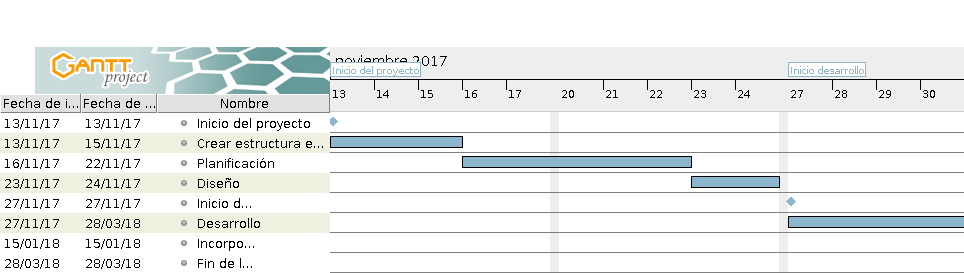
\includegraphics[angle=90,scale=0.5]{img/gantt-start}
    \caption{Diagrama de Gantt correspondiente a los hitos iniciales del
      proyecto}
    \label{fig:diag:start}
\end{figure}

\begin{figure}[h]
    \center
    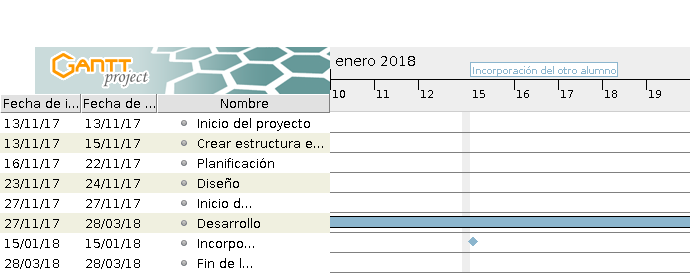
\includegraphics[angle=90,scale=0.5]{img/gantt-middle}
    \caption{Diagrama de Gantt correspondiente a los hitos hacia la mitad del
      proyecto}
    \label{fig:diag:middle}
\end{figure}

\begin{figure}[h]
    \center
    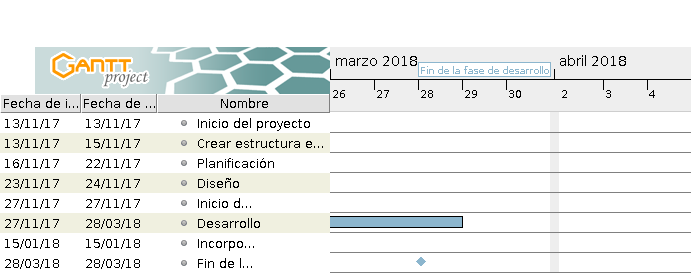
\includegraphics[angle=90,scale=0.5]{img/gantt-end}
    \caption{Diagrama de Gantt correspondiente de los hitos finales del
    proyecto}
    \label{fig:diag:end}
\end{figure}

\subsection{Seguimiento y control}
\label{subsec:syc:timeManagement}
Por los motivos especificados en la sección de planificación \ref{plan:time},
el esfuerzo de la gestión de tiempo del proyecto se realizará en este apartado.
La idea es recoger todas, o la gran mayoría de las actividades realizadas a lo
largo del proyecto, de forma que después se puedan elaborar conclusiones sobre
qué es importante estimar y qué no, en un proyecto de estas características.
